\documentclass{thesis}

\usepackage{siunitx}
\usepackage{tikz}
\usetikzlibrary {positioning,fit,calc}

\newcommand{\todo}[1]{{\color{red}TODO: #1}}

% I don't know whether to talk in first person plural or singular
\newcommand{\We}{We}
\newcommand{\we}{we}
\newcommand{\our}{our}
\newcommand{\Our}{Our}

% Units
\newcommand{\V}{\unit{\volt}}
\newcommand{\mV}{\unit{\milli\volt}}
\newcommand{\uV}{\unit{\micro\volt}}
\newcommand{\nV}{\unit{\nano\volt}}
\newcommand{\Hz}{\unit{\hertz}}
\newcommand{\kHz}{\unit{\kilo\hertz}}
\newcommand{\us}{\unit{\micro\second}}
\newcommand{\mm}{\unit{\milli\meter}}
\newcommand{\K}{\unit{K}}
\newcommand{\ohm}{\unit{\ohm}}
\newcommand{\kohm}{\unit{\kilo\ohm}}
\newcommand{\dB}{\unit{\deci\bel}}

% Signal names
\newcommand{\drdy}{{\ensuremath{\mathtt{DOUT/}\overline{\mathtt{RDY}}}}}

\addbibresource{bibliography.bib}

\begin{document}

\defaultfont

\maketableofcontents

\section{Introduction}

Electrophysiology \todo{what is}

The most prevalent\todo{cite} modes of biopotential measurements are electrocardiography (ECG) and electromyography (EMG), measuring cardiac muscle potentials and skeletal muscle potentials respectively. While methods that use intracellular electrodes exist and are much more precise \todo{cite}, using surface electrodes is very common thanks to their non invasive nature, albeit at a loss of specificity due to measuring a superposition of nearby potentials. The field of ECG is by and large applied to identifying and diagnosing cardiac abnormalities in clinical and first responder settings, focusing on disturbances of the cardiac rhythm, artery blood flow, or electrolyte availability for diagnosis of heart conditions.\todo{cite} On the other hand, Surface EMG (henceforth sEMG) has broader applications, ranging from the clinical, such as diagnosing nerve and muscle damage, to prosthetics, rehabilitation, biofeedback therapy, ergonomics, sports and movement science \cite{Barbero2012}, and it also opens up the possibility of novel Human-Computer Interaction methods.

Although the electrical design of biopotential measurement devices has been studied for hundreds of years, tracing back to Luigi Galvani's work in the 18th century, and there exist a number of current-day commercial, academic, and DIY solutions, only a small part aspire to the ideals of Open Source Hardware and/or Open Source Software (ASPEN\cite{Esposito2018}, openBCI\cite{openbci}, BioAmp-EXG-Pill\cite{pill}, MyoWare EMG\cite{myoware}), and there exist no systems that integrate with ROS2 or the Linux IIO subsystem, limiting their flexibility in terms of building software that seamlessly interfaces with them.

We aim to fill this gap and provide an affordable and easily maintainable hardware and software solution for measuring multi-channel biopotential signals and interfacing them with ROS2 and LibIIO. Adapting this system to work with other software suites should be made as simple as possible thanks to the versatility of both ROS2 and LibIIO, and adapting it to other hardware platforms should also be facilitated by the decoupled nature of the hardware, firmware and software parts.

\todo{What is ROS2}

The Linux Industrial I/O (IIO) subsystem was created in 2008 and mainlined in 2012 (\href{https://github.com/torvalds/linux/commit/06458e277eac2b8761b0a04d3c808d57be281a2e}{commit \texttt{06458e2}}) to provide a simple and unified way to interact with devices with ADC or DAC capabilities, broadly ranging from plain ADC/DAC chips to Inertial Measurement Units (Accelerometers, Gyroscopes, Magnetometers), Software Defined Radio, robotic actuators and sensors, and more. Within the Linux kernel, it fills in a gap between the \textit{input} subsystem which can stream user input data and the \textit{hwmon} subsystem used for monitoring and controlling hardware state such as CPU temperature and fan settings, albeit with low refresh rate. The IIO subsystem provides a modular way to define high bandwidth communication with input/output devices directly connected to the host via SPI or I2C and specified as part of the device tree. Despite the subsystem's name, it is not limited to industrial production applications: IIO usage is ubiquitous in today's linux-based devices for integrating features such as accelerometers, gyroscopes or ambient light sensors in a uniform way, besides other hardware abstraction layers.

\textit{Libiio} is a library which provices cross-platform functionality for interacting with both local and remote IIO devices within the same framework. To accomplish this, it implements the IIO Daemon (IIOD) for which it defines the \textit{IIOD protocol}. The current version of the IIOD protocol (v0.1) is based on a set of human readable commands sent via a single data stream of alternating client requests and server responses. This allows the same protocol to be used over a variety of transport layers, officially Serial (most relevant for this application), USB and TCP.

We present overview of the information flow, from the biological signals to the software, in figure \ref{fig:flow}.

\begin{thesisfigure}{Overview of information flow}{flow}
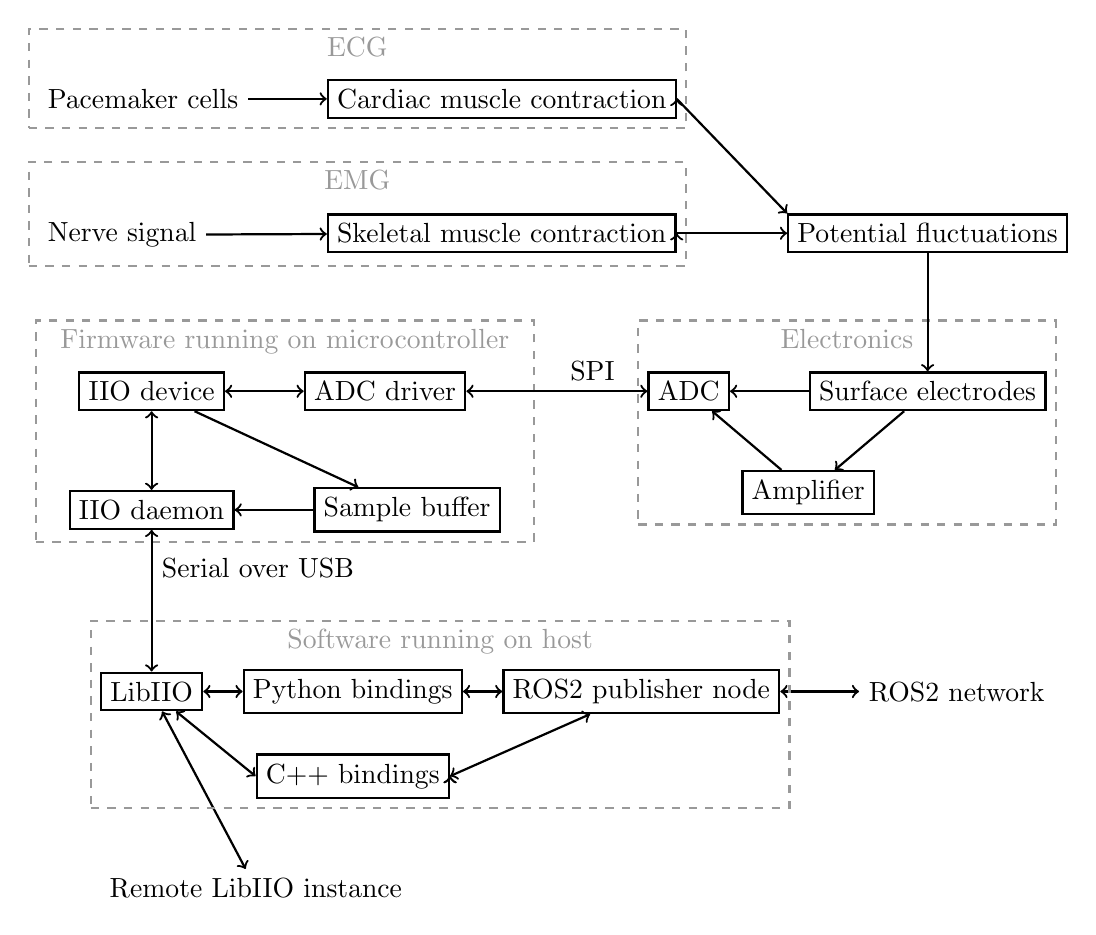
\begin{tikzpicture}[
    node distance=10mm,
    component/.style={
        rectangle, thick, draw=black
    },
    system/.style={
        rectangle, thick, dashed, draw=black!40, text=black!40
    }
]
    \node (pac) [] { Pacemaker cells };
    \node (car) [component, right=of pac] { Cardiac muscle contraction };
    \node (paccar) [fit={(pac) (car) ([yshift=1.5em]pac.north)},system,label={[text=black!40,anchor=north]north:ECG}] {};

    \node (ner) [below=12mm of pac.south west, anchor=north west] { Nerve signal };
    \node (ske) [component, below=12mm of car.south west, anchor=north west] { Skeletal muscle contraction };
    \node [fit={(ner) (ske) ([yshift=1.5em]ner.north)},system,label={[text=black!40,anchor=north]north:EMG}] {};

    \node (midcarske) at ($(car)!1!(ske)$) {};

    \node (pot) [component, right=35mm of midcarske] { Potential fluctuations };

    \draw [->, thick] (pac) edge (car);
    \draw [->, thick] (car.east) edge (pot.north west);

    \draw [->, thick] (ner) edge (ske);
    \draw [->, thick] (ske.east) edge (pot.west);

    \node (ele) [component, below=15mm of pot] { Surface electrodes };
    \node (adc) [component, left=of ele] { ADC };
    \node (amp) [component, below=of $(ele)!0.5!(adc)$] { Amplifier };

    \node [fit={(ele) (amp) (adc) ([yshift=1.5em]ele.north)},system,label={[text=black!40,anchor=north]north:Electronics}] {};

    \path [->, draw, thick]
        (pot) edge (ele)
        (ele) edge (amp)
        (ele) edge (adc)
        (amp) edge (adc);

    \node (dri) [component, left=23mm of adc] { ADC driver };
    \node (dev) [component, left=of dri] { IIO device };
    \node (iod) [component, below=of dev] { IIO daemon };
    \node (buf) [component, right=of iod] { Sample buffer };

    \node [fit={(dri) (dev) ([xshift=+3mm]buf.south east) ([xshift=-3mm]iod.west) ([yshift=1.5em]dev.north)},system,label={[text=black!40,anchor=north]north:Firmware running on microcontroller}] {};

    \path [<->, draw, thick]
        (adc) edge node[very near start,above,anchor=south east] {SPI} (dri)
        (dri) edge (dev)
        (iod) edge (dev);

    \path [->, draw, thick]
        (dev) edge (buf)
        (buf) edge (iod);

    \node (lib) [component, below=18mm of iod] { LibIIO };
    \node (pyt) [component, right=5mm of lib] { Python bindings };
    \node (cpp) [component, below=5mm of pyt] { C++ bindings };
    \node (rem) [below=25mm of lib.west,anchor=west] { Remote LibIIO instance };

    \path [<->, draw, thick]
        (iod) edge node [very near start, right, anchor=north west] {Serial over USB} (lib)
        (lib) edge (pyt.west)
        (lib) edge (cpp.west)
        (lib) edge (rem);

    \node (ros) [component, right=5mm of pyt] { ROS2 publisher node };
    \node (net) [right=of ros] { ROS2 network };

    \path [<->, draw, thick]
        (pyt) edge (ros)
        (cpp.east) edge (ros)
        (ros) edge (net);


    \node [fit={(ros) (cpp) ([yshift=1.5em]lib.north west)},system,label={[text=black!40,anchor=north]north:Software running on host}] {};
\end{tikzpicture}
\end{thesisfigure}

\newpage
\section{Bibliographic research}

% (current state of the art + problem justification + possible approaches)

\subsection{Anatomical basis}

% (car), (ske), (pot)

As part of normal function, all biological cells have a difference of electrical potential between their interior and their exterior, called the \textit{membrane potential}. In the steady state, the \textit{resting membrane potential} of both skeletal muscle cells and that of cardiomyocytes (cardiac muscle cells) is in the $\numrange{-70}{-90} \mV$ range \cite{Hopkins2006,Klabunde2011-jo}.



\todo{WIP: skeletal muscles, Sarcomere, sliding filament model, essential parts from \cite{Barbero2012}}

\todo{ECG: find a reputable source to cite for cardio physiology}

\subsection{Market research and literature review}

Biopotential measurements are no new subject and many products already exist both in the academic and commercial fields. All are subject to engineering tradeoffs between parameters such as number of channels, sample rate, precision, noise, electrode types, etc., making each better suited to a certain use case. To the best of our research, there is no universal, modular and extensible solution to the problem of biopotential measurements. Further on, we overview some representative options for EMG / ECG DAQ systems:

\subsection*{OpenBCI}

Expensive, low data rate. \todo{more :)}

\subsection*{ASPEN}

\cite{Esposito2018}

What we're doing, but better, but a PhD thesis.

\todo{more :)}


\subsection*{Quanser QNET Myoelectric board}



Depends on NI Elvis; one channel; not open \todo{more :)}

\subsection*{BioWare EXG Pills}

Just the amplification part, no DAQ, rely on an arduino's ADC or some other. \todo{more :)}

\subsection*{Cometa Pico EMG}

\href{https://www.cometasystems.com/pico-emg/}{Cometa Pico EMG}

not open, expensive\todo{more :)}


\subsection*{MyoWare}

\todo{more :)}

\subsection*{the green one I forgot the name of}

\todo{more :)}

\subsection{Noise sources}

The superposition of electrical signals measurable by biopotential DAQs contains a complicated mix of noise coming from various physiological and other external factors, besides the signal of interest. Additionally, the measurement circuitry compounds noise at every step. Modeling some of the main noise components of the entire signal chain is essential for its design.

Some of the studied noise sources are \textit{intrinsic} to the process and impossible to remove, such as thermal noise and the amplifier and ADC noise profiles. Others are not intrinsic, depend on the setup, and can be compensated for, such as mains hum.

\subsubsection{Thermal noise}

Even with ideal conductors and measurements, any resistive circuit will be affected by thermal noise, as a consequence of Planck's law of blackbody radiation \cite[chapter 3.2]{Urick2015-pm}. An ideal resistor $R$ at absolute temperature $T$ will manifest thermal noise $V_n$ over a frequency window $\Delta f$ having mean squared value \( \overline{V_n^2} = 4k_BTR\Delta f \), where $k_B = 1.380649\cdot10^{−23} \unit{J\per K}$ is the Boltzmann constant.

For a rough estimate of the order of magnitude of thermal noise in our biopotential measurements, we study the following hypothetical setup: Assume the electrodes attached to the patient are in thermal equilibrium at a typical skin temperature of $T \approx 308 \K$ \cite{Suarez2016}, we are limiting the frequency band to $\Delta f = 500 \Hz$ by filtering, and experiencing a typical resistance ${R \approx 3500 \ohm}$ (electrode + contact + internal resistance) \cite{Kurniawan2022}. This is only useful as a rough order estimation, because the resistance will vary depending on the electrode location, surface preparation, measured individual, electrode condition, etc. The estimated thermal noise will is:

\begin{thesisequation}{thnoisevalue}
\overline{V_n^2} = 4k_BTR\Delta f \approx 0.02977 \uV^2
\end{thesisequation}

Which can alternatively be interpreted as having an RMS noise of $\sqrt{0.02977 \uV^2} \approx 172.5 \nV$ or a noise density of $\sqrt{4k_BTR} = 7.716 \nV/\sqrt{\Hz}$. 

\subsubsection{Amplifier and ADC noise}

Both ADCs and amplifier circuits have specified noise figures which pose design tradeoffs. In ADCs, the noise is specified as additive noise at the input $V_{na}$, such that a measurement $V_{meas}$ of a "real" voltage $V$ will be $V_{meas} = V + V_{na}$. Amplifiers are characterized by both input noise $V_{ni}$ created by the input stage, as well as output noise $V_{no}$ created by internal circuirty and the output stage. The output of an amplifier with gain $G$ is $V_{amp} = (V + V_{ni}) \cdot G + V_{no}$. As an easier to use figure, the \textit{Input Referred Noise} is the equivalent disturbance at the input that would create both the effects of input and output noise componded. $\text{IRN} = V_{ni} + V_{no}/G$ such that we can simplify to $V_{amp} = (V + \text{IRN}) \cdot G$.

This raises one of the most important design decisions of the signal chain, namely deciding on the amplification structure before the ADC. Using no amplifier at all is the most economic and also avoids $V_{ni}$ and $V_{no}$, but in the case of very small input signals, they are left to be dominated by ADC noise $V_{na}$. Adding an amplifier with unity gain only compounds amplifier noise and is as such detrimental, but further increasing the gain increases the signal-to-noise ratio (SNR):

\begin{thesisequation}{snr}
\text{SNR} = \frac{\text{"signal"}}{\text{"noise"}} = \frac{G\cdot V}{G\cdot V_{ni} + V_{no} + V_{na}} = \frac{V}{V_{ni} + (V_{no} + V_{na}) / G} \longrightarrow \frac{V}{V_{ni}}
\end{thesisequation}

Thus, given an amplifier with known $V_{ni}$ we can compute the best-case noise figure assuming "infinite" gain. The rationally convergent nature of the above expression inevitably creates a situation of diminishing returns, wherein increasing the gain will always increase the signal quality, but even relatively small gains achieve practically ideal performance.

The drawback of having very large gain is the limit it incurs on the measurable range of input voltages. Any analog circuit can only handle a limited interval of voltages, which when exceeded leads to unreliable measurements, with the possibility of permanent damage to the equipment. If the ADC is limited to measuring $\pm V_{max}$, the measurable signals are implicitly limited to $\pm V_{max}/G$.

\subsubsection{ECG noise models}

Besides the unavoidable thermal and electronics noise, further disturbances in ECG measurements can be classified, as per \cite{Chatterjee2020}, into: low frequency ($< 0.5\Hz$) baseline wander caused by body motion and electrode contact issues, power-line artifacts ($50/60\Hz$ and their harmonics) caused by insufficient power supply decoupling when the measurement device is connected to mains power, and muscle artifacts (EMG signals). Of the three, the first two are relevant and undesireable in any biopotential measurement, while the latter is obviously the signal of interest in EMG applications.

From a signal processing standpoint, a simple solution for low frequency wander and power line artifacts is using a DC blocking comb filter.

\subsection{Signal chain design}

\todo{figure out which parts go in the background section and which go to the design section. Currently put everything in the design section.}

\subsubsection{Instrumentation amplifiers}

\subsubsection{Multiplexed ADCs}

\subsubsection{?}

\newpage
\section{Analysis, design and implementation}

\subsection{Objectives}

Additionally, we 

\todo{Justify objectives, format these boring bullet lists in a nicer way}

MUST:
\begin{itemize}
\item Open Hardware and So20ftware
\item 8 channels
\item Per-channel configuration
\item 1000Hz data rate (500Hz bandwidth) \todo{NNNNNOOOOOOOOO}
\item High CMRR, PSRR
\item High SNR (>40dB EMG; >20dB for ECG)
\item Open and extensible interfacing: ROS2, IIO
\end{itemize}

SHOULD (unchecked go to future work):
\begin{itemize}
\item 16 channels
\item Differential / single-ended configurability
\item Right Leg Drive
\item 1024Hz/2048Hz /channel data rate (1 Hz per FFT bin)
\item <1uV noise after filtering
\item 1uV precision
\end{itemize}

Guiding principles:
\begin{itemize}
\item Cost
\item Usability as an educational tool
\item Use Analog Devices parts
\item Modularity (decoupled hardware-firmware-software)
\end{itemize}

\todo{After finishing the prototype, make a comparison table between the already existing products and mine, especially on these objectives}

\todo{Signal chain figure:
1. Patient, anatomy
2. Electrodes
3. Buffer and amplification
4. ADC
5. Microcontroller, using the no-OS framework. Contains customizable digital filters
6. IIO protocol
7. Linux IIO subsystem
8. libiio, pyadi-iio
variant A, with a network-enabled microcontroller:
from 5, ROS2 protocol {find the name!} to ROS2 network running on the microcontroller
variant B, with a microcontrollwe without networking capabilities:
from 8, ROS2 protocol to ROS2 network running on the carrier board / host}

\newpage
\subsection{Electical part}

\subsubsection{Interfacing with the patient}

The first step we control in the signal chain is the point of contact with the patient. The electrode type and quality have a great influence on the overall design, performance, and subjective user experience.

The state of the art are conductive polymer PEDOT:PSS electrodes, thanks to their great mechanical, electrical, and chemical properties: They adhere and conform to skin, are flexible, self-healing, and have good biocompatibility, only falling behind the classic Ag/AgCl electrodes in terms of contact impedance, yet still being conductive enough for biopotential readings. \cite{Seiti2023,Hou2024} We do not consider them viable for this project due to them not being commercially available in standard and mass produced forms, being mostly a custom product experimented with in today's laboratories, even half a century after their discovery in the 1980s.

DIY cheap alternative \todo{cite that paper with DIY AgCl electrodes}

This project settles for snap-on adhesive ECG gel electrodes thanks to being cheap, readily avaialble, standardized, and they can be connected to with inexpensive aligator clips, besides special (but more expensive) snap clips. The downsides are their low shelf life \todo{compare expired electrode signal quality with fresh electrodes once I get some fresh ones}, comparatively larger contact area (cca $200\mm^2$ vs \cite{Barbero2012}'s 2mm electrode diameters), and are lacking in subjective user experience, sometimes being very painful to detach.

\subsubsection{ADC}

\todo{preface on how to choose an ADC}

We initially chose the AD7124-8\cite{AD7124-8} thanks to its very diverse feature set, including: programmable gain amplifiers (PGAs) which had the potential to remove the need for the external amplification stage, high precision, high number of channels, and high sample rate. Unfortunately, it is not a single cycle ADC. This means that although it has very good throughput on a single channel, when switching between two channels there is a dead time for the integrated filter to settle, which effectively reduces the per-channel sample rate to less than $100\Hz$ when sampling all 16, which is virtually useless for ECG ($f_\text{max}=150\Hz$) and EMG ($f_\text{max}=500\Hz$).

Our next choice was the AD4114\cite{AD4114}. It doesn't include PGAs, but otherwise has very good specs and has a much higher sample rate and a single cycle conversion mode.

\todo{spec comparison between AD7124-8 and AD4114?}

\todo{describe AD4114 function, especially: channels vs setups, internal channel sequencer, overall communication model, \textbf{how to check for new samples}, noise versus sample rate. All of these will more or less paraphrase the datasheet.}

\todo{$1007\Hz$ and $6211\Hz$ are the sample rates we're most interested in}

\subsubsection{Amplification stage}

The chosen AD4114 ADC has $N=24$ bits of resolution with one LSB equating to $\Delta v \approx 1.49\uV$ if using the internal $2.5\V$ reference. At $f_s=1007\Hz$ and $f_s=6211\Hz$, the ADC noise is specified to be around $\overline{V_{na,1007}^2}=20\uV$ and $\overline{V_{na,6211}^2}=74\uV$ RMS respectively. Without an amplification stage, this would result in the following SNRs:

\begin{thesisequation}{SNR_no_amp}
\begin{aligned}
\text{SNR}_{(\dB)} &= 10\log_{10}\left(\frac{(1\mV)^2}{\overline{V_{na}^2}}\right) \\
\text{SNR}_{1007} &\approx 34\dB \\
\text{SNR}_{6211} &\approx 23\dB 
\end{aligned}
\end{thesisequation}

We choose the AD8226 \cite{AD8226} instrumentation amplifier for the preamp stage. It is inexpensive, readily available, has more than sufficient CMRR ($>80\dB$) and can be configured for a gain of $G=\numrange{1}{1000}$ using a resistor $R_G = 49.4\kohm / (G-1)$. Its RMS voltage noise for our desired bandwidth $\Delta f=500\Hz$ is:

\begin{thesisequation}{8266_noise}
\begin{aligned}
V_{ni,RMS} = \sqrt{500\Hz \cdot (22\nV/\sqrt{\Hz})^2} = 0.492\uV \\
V_{no,RMS} = \sqrt{500\Hz \cdot (120\nV/\sqrt{\Hz})^2} = 2.683\uV
\end{aligned}
\end{thesisequation}

With the preamp stage added before the ADC, the total noise of a sample and the theoretical SNR ($1\mV$ input) are:

\begin{thesisequation}{noise_amp}
\begin{aligned}
\overline{V_n^2} = \overline{V_{ni}^2} + \frac{\overline{V_{no}^2} + \overline{V_{na}^2}}{G^2} \\
\text{SNR}_{(\dB)} = 10\log_{10}\left(\frac{(1\mV)^2}{\overline{V_{n}^2}}\right)
\end{aligned}
\end{thesisequation}

An illustrative handful of values for various gain settings: \todo{rephrase :)}

\begin{thesistable}{0.33}{l|ll}{a}{b}
Gain & Full scale & $\text{SNR}_{(\dB)}$ \\ \hline
1    & $5\V$      & $34\dB$ \\
2    & $2.5\V$    &  $40\dB$ \\
5    & $1\V$      &  $48\dB$ \\
10   & $500\mV$   &  $54\dB$ \\
20   & $250\mV$   &  $59\dB$ \\
50   & $100\mV$   &  $64\dB$ \\
100  & $50\mV$    &  $65\dB$ \\
1000 & $5\mV$     &  $66\dB$ \\
\end{thesistable}







- adc has 24 bits of resolution => ? uV LSB => would seem like it's already suitable for our measurement ranges. Compute number of bits and SNR given a known ECG, EMG amplitude.
- but we can do better! A pre-amp stage will amplify the signal, add some noise, but ultimately reduce the IRN.
- can't amplify too much, though, because we don't want to exceed the full scale (or really the 0-5V supply for that matter)
- set a hard limit for the gain so we don't clip
- compute bits / SNR for some gain values (as well as for no amplifier)
- plot or table showing diminishing returns. Just stop when we're <0.5-1 bits from the best we can do (gain=1000)

\todo{tikz figure of signal chain}

Assuming a single , followed by an ADC input noise $V_{na}$, are measuring the "true" voltage $x$, the resulting digitized sample $y$ can be decomposed into:

\begin{thesisequation}{decomposey}
y = Gx + GV_{ni} + V_{no} + V_{na}
\end{thesisequation}

Which can be rearranged to obtain an expression for RMS total noise $V_n^2$:

\begin{thesisequation}{rmsnoise}
\overline{x^2} = \frac{\overline{y^2}}{G^2} + \underbrace{\left(\overline{V_{ni}^2} + \frac{\overline{V_{no}^2} + \overline{V_{na}^2}}{G^2}\right)}_{\overline{V_n^2}}
\end{thesisequation}







\subsubsection{Microcontroller}

The chosen microcontroller platform is the MAX78000FTHR.

Main requirements for the microcontroller:
- SPI rate high enough to read the ADC at the wanted sample rate
- Enough CPU freq and memory to run the IIO Daemon.

Nice-to-haves:
- Networking capabilities so it can run a ROS2 node as a standalone device, not needing another "carrier" to forward the data to the ROS network.

Suitable very cheap microcontrollers:
- ESP8266, ESP32
- RP2040 based boards (Raspberry Pi Pico, GroundStudio Pico, other clones)

The popular (yet more and more obsolete) ATMEGA328p of Arduino fame isn't fast enough for recording and further transferring all 16 channels. Especially not with a non-custom IIOD / ros-micro implementation.

\newpage
\subsection{Firmware part}

\todo{Short 100-200 word intro about firmware}

\todo{The no-OS framework}

\todo{What is No-OS and why do \we use it? Main points: more than a Hardware Abstraction Layer; decouples hardware platforms, peripherals, libraries. While it adds an initial development overhead, it helps a lot with porting the firmware to other boards, sensors, or even software communication schemes.}

\subsubsection{Serial communication with host}

In order to send data to the attached computer or carrier board, the de facto solution is using UART-over-USB, which exposes an USB interface to the attached host and UART to the microcontroller. Most commonly, microcontrollers have dedicated circuitry for UART transmit and receive, which allows the rest of the program to run concurrently to serial communication. This is implemented using two FIFO buffers, one for data pending to be sent from the microcontroller (TX FIFO) and one for received data ready to be processed by the program (RX FIFO).

De facto, most microcontroller development boards, including the MAX78000FTHR, MAX-Arduino, and the more common ATMEGA368P "Arduino-like" boards provide UART-USB translation via a dedicated IC, abstracting away the complexities of the USB communication stack.

UART modules have varying degrees of configurability of the baud rate, flow control, and framing. For most practical uses, though, including this project, one may just specify the baud rate, defaulting to 8N1 (8 data bits, no parity bit, 1 start bit, 1 stop bit) framing and no flow control. Typical baud rates include 9600 baud, a legacy of 20th century POTS modems (introduced by the V.32 ITU-T standard \cite{}) and 115200 baud, common both in last-century modem systems, but also recently popularized by its default use in the Arduino development environment.

To achieve the required bandwidth for this project, a suitable baud rate must be chosen. Given the sample rate $f_s$, number of channels $N$, and number of bytes per channel sample $d$, and 8N1 framing (giving $10\text{ baud}/\text{byte}$), the baud rate $f_{baud}$ must be:

\begin{thesisequation}{baud}
f_{baud} \geq f_s \cdot N \cdot d \cdot 10 = 1024 \cdot 16 \cdot 3 \cdot 10 = 491520\text{ baud}
\end{thesisequation}

Additionally, choosing a baud rate larger than this minimum will allow for less timing concerns, especially when it comes to not overflowing the receive and transmit buffers.

Baud rate selection is not universal across devices and the firmware for each hardware platform must choose a rate that is both compatible with the hardware and that satisfies relation \ref{eq:baud}. In the case of the MAX78000FTHR, a rate of exactly $491520\text{ baud}$ can be achievend by using the IBRO (Internal Baud Rate Oscillator) of $7.3728\text{MHz}$ with a clock divider of $15$, but [we] will use a divider of $9$ for a "round" value of $819200\text{ baud}$ to have a good margin of error and not need such strict synchronization between the UART module and the rest of the program.

\subsubsection{SPI Communication basic proof of concept (2024-05 single channel demo)}

For initial validation of the concept on the AD4114, \todo{write about the PoC: 1 channel, no amplification, full sample rate, can see both EMG and ECG on it. can do nice graphs, can diagnose my RBBB}

\subsubsection{No-OS Driver}

For easy portability to different microcontroller platforms and even other ADCs, I'm using the No-OS framework, which facilitates separating the general logic from product-specific code and settings.

\subsubsection{IIOd integration}

Defining the structure of the IIO context is a very important step as it solidifies a mapping between the device-specific functionality on the hardware side and the application-specific functionality on the software side. Choosing a versatile collection of attributes to configure the device and channels to structure the data is no trivial task with no unique solution. The exposed attributes may encode very low level details, as in {find an AD part with a very bare-metal attribute mapping}, or more high level ones. Choosing which configuration is to be specified on the software side and which configuration is to be derived from that on the firmware side {of pula mea ce scriu aici... vreau sa zic ca nu o sa expun direct registri, ci o sa expun chestii mai high level: frecventa de mains hum (50/60), parametri de filtrare, poate sample rate daca o sa imi dau variante (posibil tho sa fie fix la 1k), si pe baza lor se ocupa firmware sa puna registrii cum trebuie.

For lower-level functionality, an IIO debug interface is also specified, which allows for direct manipulation of the ADC's registers. This shouldn't be normally used, but allows for total control of the device in case the user needs it.

1. Defining the desired iio context structure: what do we expose, in which formats, etc
2. Handler functions
3. Boom done, connect to it from software

\subsubsection{Continuous and asynchronous data acquisition using IIO triggers}

By default, the expected behaviour of IIO devices is to start acquisition on selected channels when requested (via an \texttt{OPEN} command), and stop and disable the channels once the requested number of samples is reached. In low sample rate scenarios, the host may request the next acquisition window very soon after the current one finishes, and assuming the time delay between windows can be minimized with respect to the overall window size, this could prevent missing any samples and only introduce a small amount of phase drift. Additionally, there are high-speed applications in which continuity between acquisition windows is not strictly required. On the other hand, with \our roughly $16\kHz$ sample rate (cca. $60 - 62\us/\text{sample}$) and requirement to not miss any samples, this application has very little room for error in timing. As per \cite{linuxlatency}, modern real-time linux setups have scheduler latencies in the tens and hundreds of microseconds, which realistically leaves no time to actually receive the current window's buffer and send a new acquisition request without missing any samples, even if the acquisition channels were left enabled.

\todo{figure, vertical stack of sequence diagrams of: normal iio polling with phase drift in slow ADC, fast ADC - loss of samples, trigger and buffer}

With this general issue in mind, IIO defines triggers as software or hardware events that initiate data acquisition without requiring regular polling from the host. Data captured as a result of triggers is stored in circular buffers and provided with minimal latency whenever the host polls next.

With the AD4114 in continuous conversion mode, two trigger sources are apparent: using the \drdy\ behaviour in continuous conversion mode (as described in \ref{label:drdy}) or using a timer to poll the AD4114 at least as fast as the conversion rate. While the first option is more elegant and wouldn't do any unnecessary polling, it requires nonstandard operation of the SPI protocol by keeping CS active and monitoring the MISO (\drdy) line, which isn't generally possible unless \we bitbang the SPI protocol or have access to more configurable IO options like on FPGA platforms or the Programmable Input and Output subsystem of RP2040 fame (\cite{Smith2021}). The second option of setting up a timer interrupt which polls the AD4114 status register to check if a new conversion result is available

\todo{more :)}

\subsubsection{ROS2 on network-capable microcontrollers}

In recent years, there has been a wave of developments in fast, network-capable, cheap microcontroller platforms, leading to products such as the Espressif ESP8266 and ESP32, or the Raspberry Pi Pico-W, which are capable of running ROS2 nodes all by themselves. 

\todo{more :)}

\subsubsection{Digital filtering of the signal}

Although the digital signal processing part of such biopotential measurement systems is very important for a full product, it is not the main topic of this thesis, and yet the chosen system architecture offloads most of the signal conditioning to the digital domain. The main source of noise is mains hum, with a fundamental frequency of $50\Hz$ and various harmonics, which can all be removed using a notching filter, resulting in minimal loss of information in other portions of the frequency spectrum. The Qaulity factor $Q$ of the filter controls how narrow the attenuated frequency bands are, and it can be adjusted. It poses a tradeoff between good noise rejection and signal quality, and is designed to be adjustable. Experimentally, we found values of around 5-10 to give the best waveforms for visual inspection. Figure X illustrates the tradeoff between small Q doing ??? and high Q doing ???.

Taking from scipy's implementation of an IIR Notching filter (`scipy.signal.iircomb`), I also use the structure described in {cite: Sophocles J Orfanidis, "Introduction to Signal Processing", Prentice-Hall, 1996, ch. 11, "Digital Filter Design"} thanks to its adjustable Q factor, numerical stability even at higher orders, and default rejection of the DC component of the signal, which are all very useful for the required signal conditioning. Parametrized by the the sampling frequency $f_s$, the cutoff freqiency $f_0$ (which must be an integer divisor of $f_s$), quality factor $Q$, the IIR filter $H(z)$ is computed as:

\begin{gather*}
N = f_s / \omega_0 \overset{!}{\in} \mathbb{N} \\
\omega_0' = \frac{2\pi\omega_0}{f_s}  \\
\omega_\Delta = \frac{\omega_0'}{Q}  \\
\beta = \tan(N * \omega_\Delta / 4)  \\
a = \frac{1 - \beta}{1 + \beta}
\end{gather*}
\begin{thesisequation}{filter}
H(z) = \frac{1}{1 + \beta} \cdot \frac{1 - z^{-N}}{1-az^{-N}}
\end{thesisequation}

\todo{check I transcribed these correctly and actually implement them myself! I only blindly copied these for now}

\newpage
\subsection{Software part}

\subsubsection{ROS2 agent for non network-capable microcontrollers}

In the case of microcontroller platforms that aren't network capable, including the MAX78000FTHR, the device itself won't have a means of directly connecting to the ROS2 network as a node. As such, it needs to pass along the data to another device that can. Two implementation variants are immediately evident: Using the micro-ROS framework, letting ros logic take over the serial device instead of having it communicate using the IIO protocol, and running a ROS-micro agent on the host
- Using the ros-control framework and an IIO-ROS2 adapter on the host / carrier board.

Of which I chose the second because it doesn't require reconfiguring the serial port and allows for simultaneous use of ROS and IIO.

\todo{implement :)}

\subsubsection{libiio, pyadi-iio}

ROS is for robotics, what about just doing some basic signal processing in python without setting it up as a ros node? Libiio has got you covered! Pyadi-iio adds a cherry on top, exposing the entire system as a very simple to initialize and query python object.

\todo{implement :)}

\newpage
\section{Results and validation}

To test the performance of the system:

- ECG is more difficult and as such a greater achievement. It has smaller amplitudes and very well-defined features, requiring more care all across the signal chain. 
- EMG is the main goal of the project, but it is more forgiving, because:
    - The signal has greater amplitude (about 10x? check both sources and experimental data!!!)
    - The signal features are not as well defined and are usually modeled like noise for signal processing.

\subsection{Electrical validation}

Using a waveform generator, we can compare this device's measurements with both:
- Precision oscilloscope readings
- Another biopotential DAQ system (Tassos')

\todo{more :) :)}

\subsection{Usage for EMG}

\todo{more :) :)}

\subsection{Usage for ECG}

\todo{more :) :)}

\subsection*{Usage for EEG???}

\todo{This would just be a cherry on top if I really don't have anything left to do in the last few days. A cool experiment would be trying out a quick and dirty \href{https://en.wikipedia.org/wiki/N100}{N100} demo. Could have a handful of visible targets on the screen, have some orthogonal and time-uncorrelated activations for each, correlate EEG (single ended frontal-occipital) with each of the PRBS to determine which target the user is focusing on}

\newpage
\section{Conclusion}

We present a hardware + software solution for biopotential measurements of up to 16 single-ended or 8 differential channels, with \todo{specs}, intended for easy and affordable maintainability, using off-the-shelf components and open source hardware and software, and being fit for 

\subsection{Future work}

Among initial ambitions which unfortunately 

\newpage
\section{Acknowledgements}

- Mark Thoren

\section{Bibliography}

\printbibliography[heading=none]

\end{document}
